\documentclass[aspectratio=169]{beamer}
\usetheme{simple}
\usepackage[english]{babel}
\usepackage[utf8]{inputenc} 
\usepackage{lmodern}
\usepackage{ragged2e}
\usefonttheme[onlymath]{serif} 
\usepackage[scale=2]{ccicons} 
% \setbeamertemplate{caption}[numbered]
\usepackage{copyrightbox}

\usepackage{graphicx,hyperref,url,pgfplots}
\usepackage{amsmath} 
\usepackage{array,booktabs}
\pgfplotsset{compat=1.13}
\usepackage{bibentry}
\usepackage[alf,abnt-etal-list=0,abnt-etal-cite=2]{abntex2cite}
\usepackage[normalem]{ulem}

\usepackage[
    type={CC},
    modifier={by-nc-sa},
    version={4.0},
]{doclicense}

\setbeamercovered{invisible} 
% \newcommand{\pausar}{\pause}
\newcommand{\pausar}{\pause}
\newcommand{\df}[1]{\,\mathrm{d}#1}
\newcommand{\parcial}[3]{\dfrac{\partial^{#1}#2}{\partial #3^{#1}}}
\newcommand{\cpright}[2]{\copyrightbox[b]{#1}{\tiny Source: #2}}

\usepackage{tikz}
\usetikzlibrary{automata,positioning}
\usepackage{xcolor}
\usetikzlibrary{scopes}
\usepackage{verbatim}
\usetikzlibrary{patterns}

\usepackage{listings}
  \lstdefinestyle{ascii-tree}{
    literate={├}{|}1 {─}{--}1 {└}{+}1 
  }
	\definecolor{codegreen}{rgb}{0,0.6,0}
	\definecolor{codegray}{rgb}{0.5,0.5,0.5}
	\definecolor{codepurple}{rgb}{0.58,0,0.82}
	\definecolor{backcolour}{rgb}{0.92,0.92,0.92}
	\lstset{language=Python, 
	backgroundcolor=\color{backcolour},   
	commentstyle=\color{codegreen},
	keywordstyle=\color{magenta},
	numberstyle=\tiny\color{codegray},
	stringstyle=\color{codepurple},
	basicstyle=\fontsize{8}{11}\ttfamily,
	frame=lines,
%	numbers=left,
	tabsize=2,
	morekeywords={models, lambda, forms},
	showstringspaces=false}


% --------------------------------------------------------------------------------------------

\title{Mobile Robots}
\subtitle{Modern Robotics}
\date{\today}
\author[Jeferson José de Lima]{
  \textbf{Professor}: Jeferson José de Lima}
\institute{Academic Department of Informatics (DAINF) \\ Federal University of Technology - Paraná (UTFPR) at Pato Branco, PR, Brazil}

\begin{document}
\maketitle
\justify


\begin{frame}{Useful Information}

	\begin{block}{License}
        \doclicenseThis
    \end{block}

	\begin{block}{links:}
		\begin{enumerate}
			\item \href{https://moodle.utfpr.edu.br/course/view.php?id=14218}{Moodle}
			\item \href{https://gitlab.com/cursoseaulas/robotica-movel/-/wikis/home}{Mobile Robots - Gitlab Page}
		\end{enumerate}
	\end{block}
\end{frame}


\begin{frame}{Modern Robots}
	\framesubtitle{\textcolor{purple}{What is Industrial Robot?}}
	\centering
	\cpright{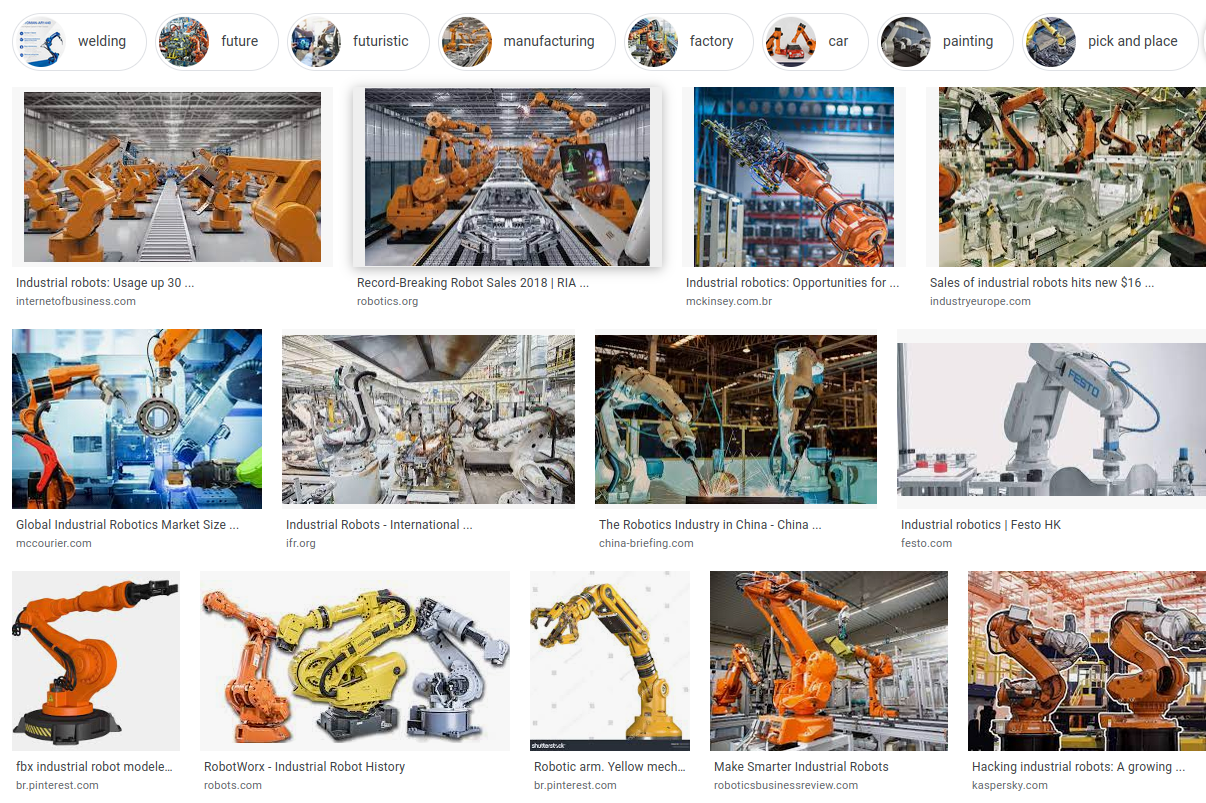
\includegraphics[width=0.7\textwidth]{./images/industrialrobots.png}}
    {https://www.google.com/search?q=Industrial+robot}

\end{frame}

\begin{frame}{Modern Robots}
	\framesubtitle{\textcolor{blue}{Robots Change the Way We Work!}}
	\centering
	\cpright{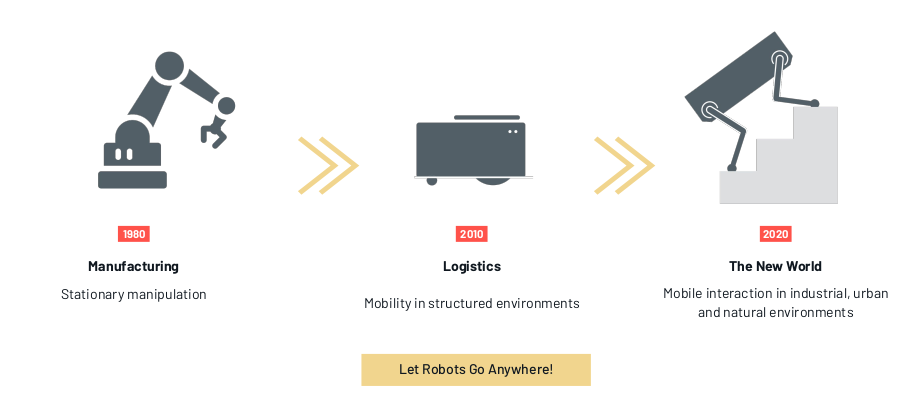
\includegraphics[width=0.8\textwidth]{./images/robots_evolution.png}}
    {https://www.google.com/search?q=Industrial+robot}
\end{frame}


\begin{frame}[fragile]{Modern Robots}
	\framesubtitle{\textcolor{purple}{ANYmal C} - Case-Based Learning}

	\begin{minipage}{0.5\textwidth}
        \cpright{\href{https://www.anybotics.com/anymal-legged-robot/}
        {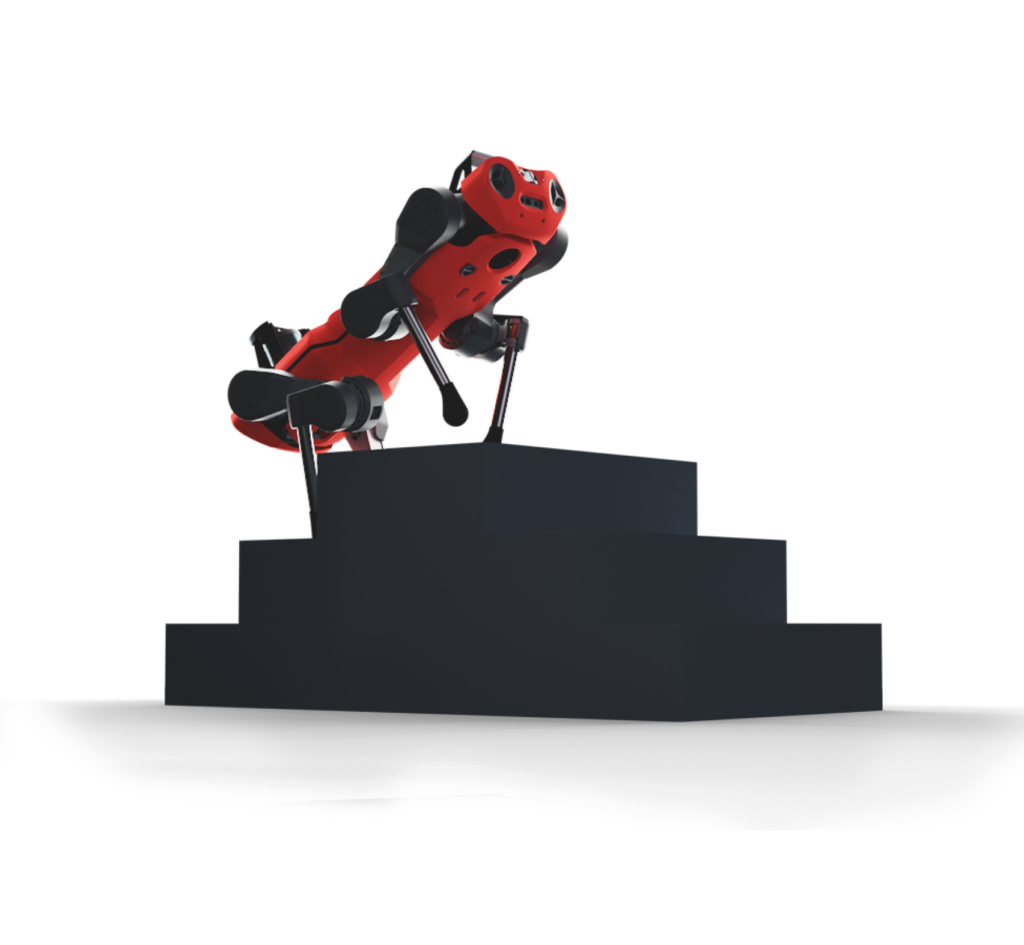
\includegraphics[width=1\textwidth]{./images/ANYmal.png}}}
        {https://www.anybotics.com/anymal-legged-robot/}
    \end{minipage}
    \begin{minipage}{0.5\textwidth}
        \begin{itemize}
            \item \textcolor{purple}{\textbf{Advanced Sensing}}:
            \begin{itemize}
                \item Obstacle Detection;
                \item Environment Scanning;
                \item Wide-Angle Cameras;
                \item GPS
            \end{itemize}
            \item \textcolor{purple}{\textbf{Full autonomy}}:
            \begin{itemize}
                \item Autonomous Path Planning;
                \item Obstacle Avoidance;
                \item Real-Time Motion Planning;
                \item Human Detection
            \end{itemize}
            \item \textcolor{purple}{\textbf{Docking station}}:
            \begin{itemize}
                \item Battery run time: $> 2h$;
                \item For full charge:  $3h$;
            \end{itemize}
            \item \textcolor{purple}{\textbf{Ease of use}}:
            \begin{itemize}
                \item Joystick;
                \item Workstation;
            \end{itemize}
        \end{itemize}
    \end{minipage}
\end{frame}

\begin{frame}[c]{Modern Robots}
	\framesubtitle{\textcolor{purple}{ANYmal C} - Evolution}
    \vspace{0.1in}
    \cpright{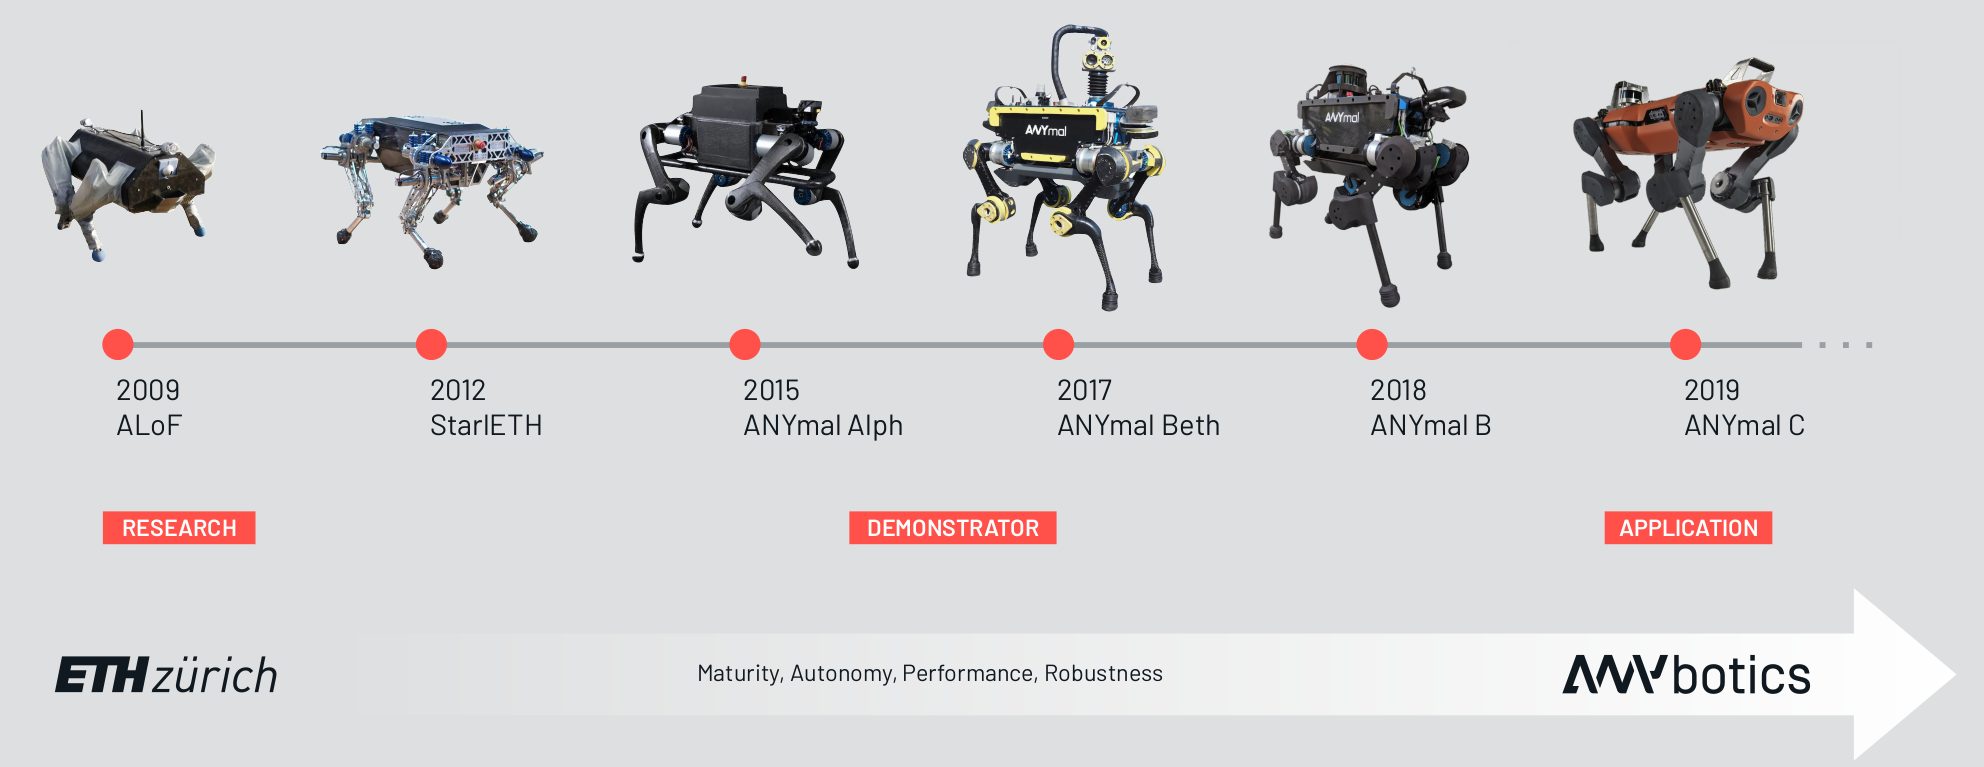
\includegraphics[width=1\textwidth]{./images/eth_ANYmal.png}}
    {https://www.anybotics.com/anymal-legged-robot/}

\end{frame}

\begin{frame}[c]{Modern Robots}
	\framesubtitle{\textcolor{purple}{ANYmal C} - Sensors}
    \vspace{0.1in}
    \cpright{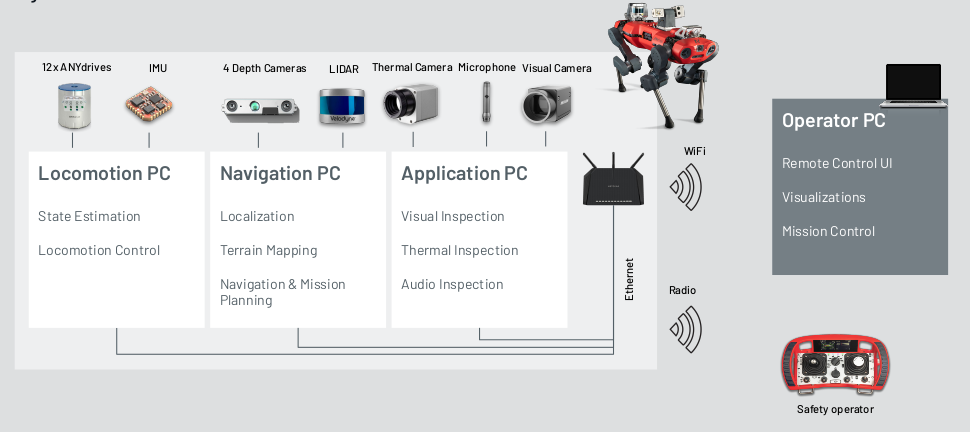
\includegraphics[width=1\textwidth]{./images/ANYmal_sensores.png}}
    {https://www.anybotics.com/anymal-legged-robot/}
\end{frame}


\begin{frame}[fragile]{Modern Robots}
	\framesubtitle{\textcolor{purple}{ANYmal C} - IMU Sensors}
	\begin{minipage}{0.3\textwidth}
        \cpright{\href{https://www.anybotics.com/anymal-legged-robot/}
        {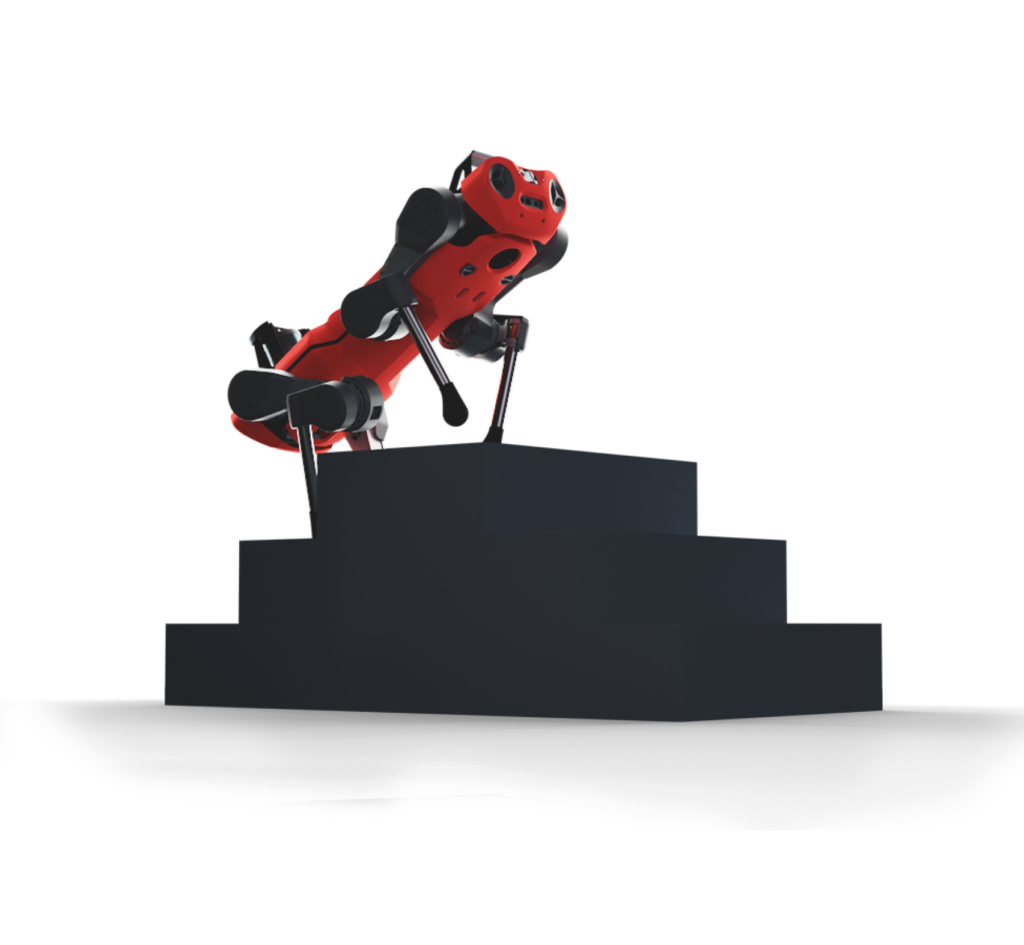
\includegraphics[width=1\textwidth]{./images/ANYmal.png}}}
        {https://www.anybotics.com/anymal-legged-robot/}
    \end{minipage}
    \begin{minipage}{0.7\textwidth}
        \textcolor{purple}{\textbf{IMU ([I]nertial [M]easurement [U]nit)}}:
        \begin{itemize}
                \item An inertial measurement unit (IMU) is a device that uses gyroscopes and accelerometers to
                estimate the relative position, velocity, and acceleration of a moving vehicle.
            \end{itemize}
            \cpright{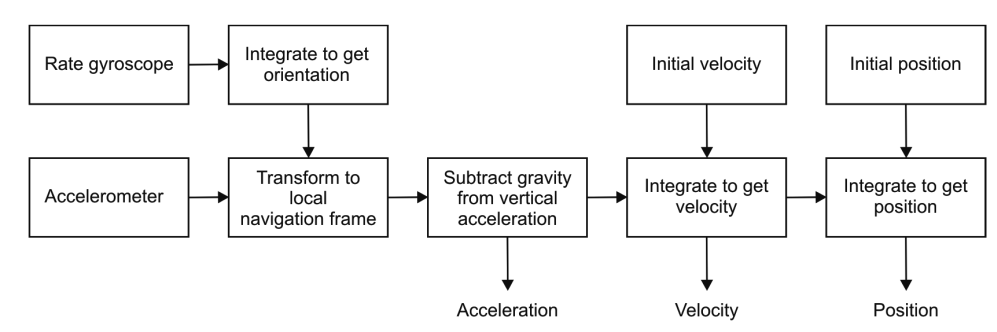
\includegraphics[width=1\textwidth]{./images/anyIMU.png}}
            {\cite{siegwart2011introduction}}
    \end{minipage}
\end{frame}

\begin{frame}[fragile]{Modern Robots}
	\framesubtitle{\textcolor{purple}{ANYmal C} - IMU Sensors}
	\begin{minipage}{0.3\textwidth}
        \cpright{\href{https://www.anybotics.com/anymal-legged-robot/}
        {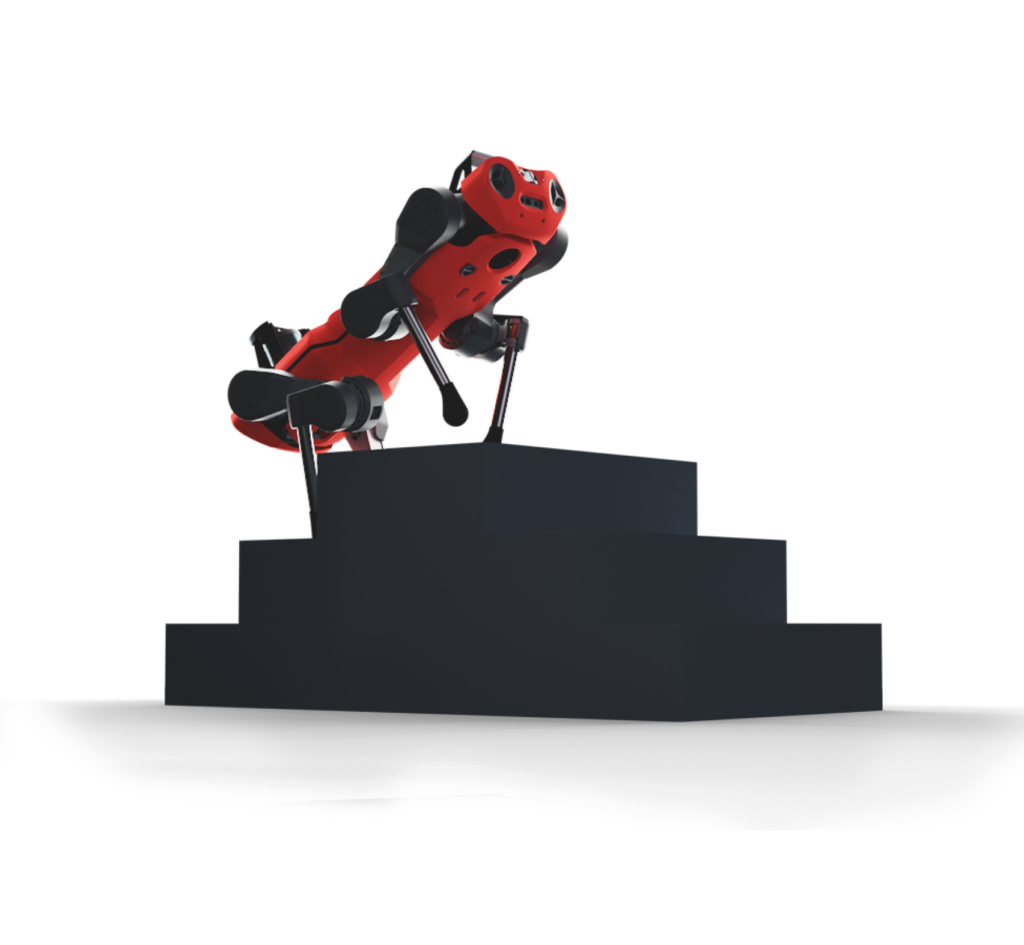
\includegraphics[width=1\textwidth]{./images/ANYmal.png}}}
        {https://www.anybotics.com/anymal-legged-robot/}
    \end{minipage}
    \begin{minipage}{0.7\textwidth}
            \textcolor{purple}{\textbf{IMU ([I]nertial [M]easurement [U]nit)}}:
            \begin{itemize}
                \item Modern accelerometers and gyroscopes are often small [M]icro [E]lectro-[M]echanical [S]ystems (MEMS);
            \end{itemize}
            \begin{figure}
                \cpright{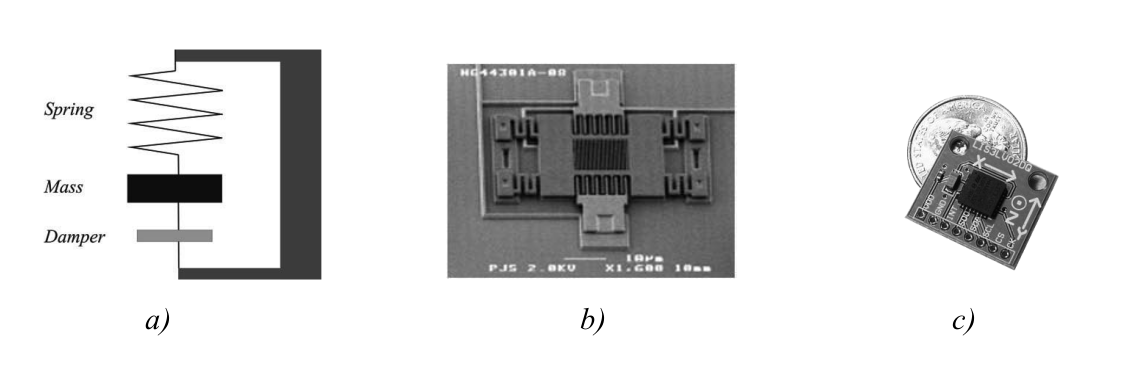
\includegraphics[width=1\textwidth]{./images/anyIMEMS.png}}
                {\cite{siegwart2011introduction}}
                \caption{(a) Working principle; (b) An example MEMS accelerometer; (c) An example commercial MEMS accelerometer.}
            \end{figure}
    \end{minipage}
\end{frame}


\begin{frame}[fragile]{Modern Robots}
	\framesubtitle{\textcolor{purple}{ANYmal C} - IMU LIDAR}
	\begin{minipage}{0.3\textwidth}
        \cpright{\href{https://www.anybotics.com/anymal-legged-robot/}
        {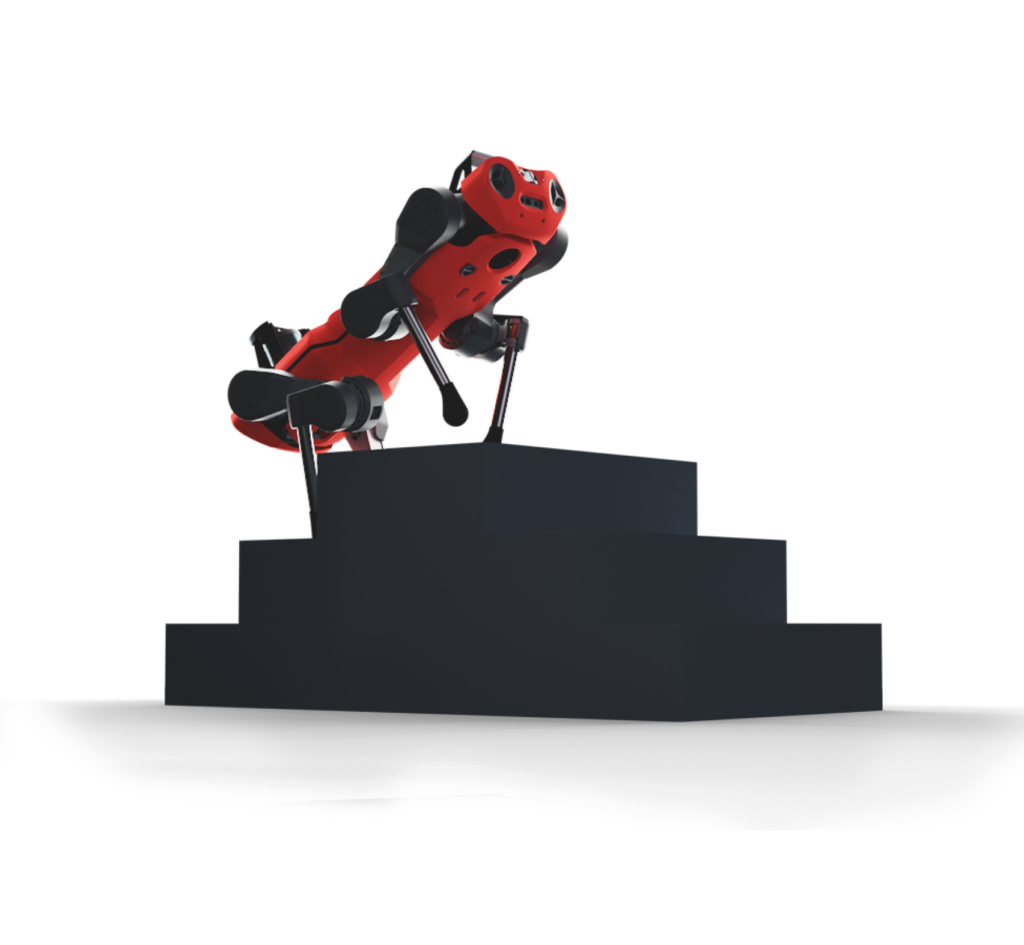
\includegraphics[width=1\textwidth]{./images/ANYmal.png}}}
        {https://www.anybotics.com/anymal-legged-robot/}
    \end{minipage}
    \begin{minipage}{0.7\textwidth}
            \textcolor{purple}{\textbf{LIDAR ([LI]ght [D]etection [A]nd [R]anging)}}:
            \begin{itemize}
                \item LIDAR devices produce a range estimate based on the time needed for the light to reach the target and return.
            \end{itemize}
            \begin{figure}
                \cpright{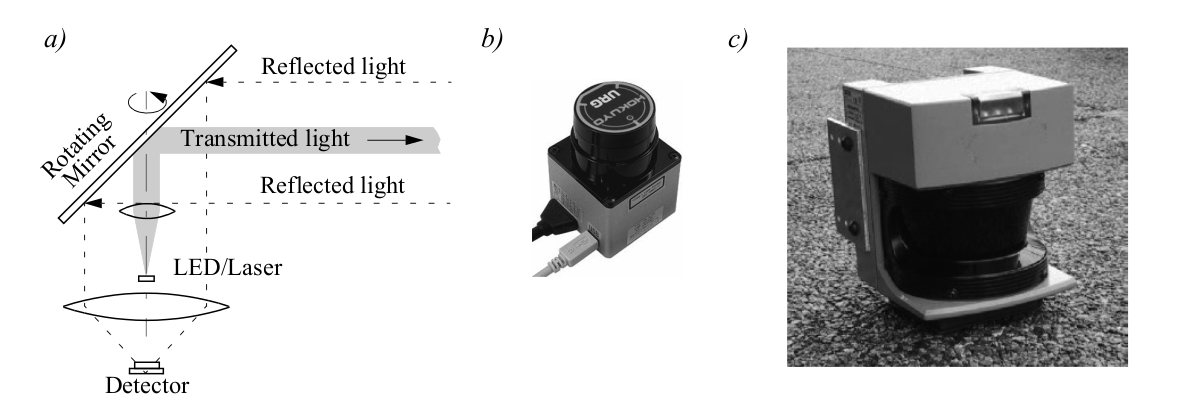
\includegraphics[width=0.9\textwidth]{./images/ANYmal_LIDAR.png}}
                {\cite{siegwart2011introduction}}
                \caption{(a) Schematic drawing of laser range sensor; (b) 240-degree laser rangefinder; (c) Industrial 180 degree laser range sensor.}
            \end{figure}
    \end{minipage}
\end{frame}


\begin{frame}[t, allowframebreaks]
	\frametitle{References}
	\bibliography{../references.bib}
\end{frame}

\end{document}